\subsection{Numerical Approximation}\label{numerical approximation}

The problem solved in the subsection~\ref{analytical results} is
defined in the continuous-space and continuous-time, and all the
analytical results are in the form of the infinite series involving
continuous variables, which will be approximated numerically in this
subsection. Moreover, for simplicity, a specific kind of annulus, with
the radius ratio $\mu=2$, is considered.

The analytical $u(\hat r, \theta, \tau)$, $S(\tau)$, and
$\langle \tau \rangle$ are in connection with the positive integers
$\lambda_{0,n}$, so the preliminary step of the numerical evaluation
is to calculate the monotonically increasing eigenvalues in
Eq.~\ref{eq:eigenfunction}.  The Figure~\ref{fig:F0} reveals the
monotonicity and periodicity of the $\lambda_{0,n}$. More precisely,
the $n$th positive zero $\lambda_{0,n}$, as $n \rightarrow \infty $,
can be bracketed in an interval $((n-1) \pi,
(n+1) \pi)$ \cite{NIST:DLMF}. Therefore, the bisection
method \cite{2020SciPy-NMeth}, a well-known and most reliable root
finding method, is used to close in on the $\lambda_{0,n}$ by
successively halving the interval until it becomes sufficiently small.

\begin{figure}
\centering
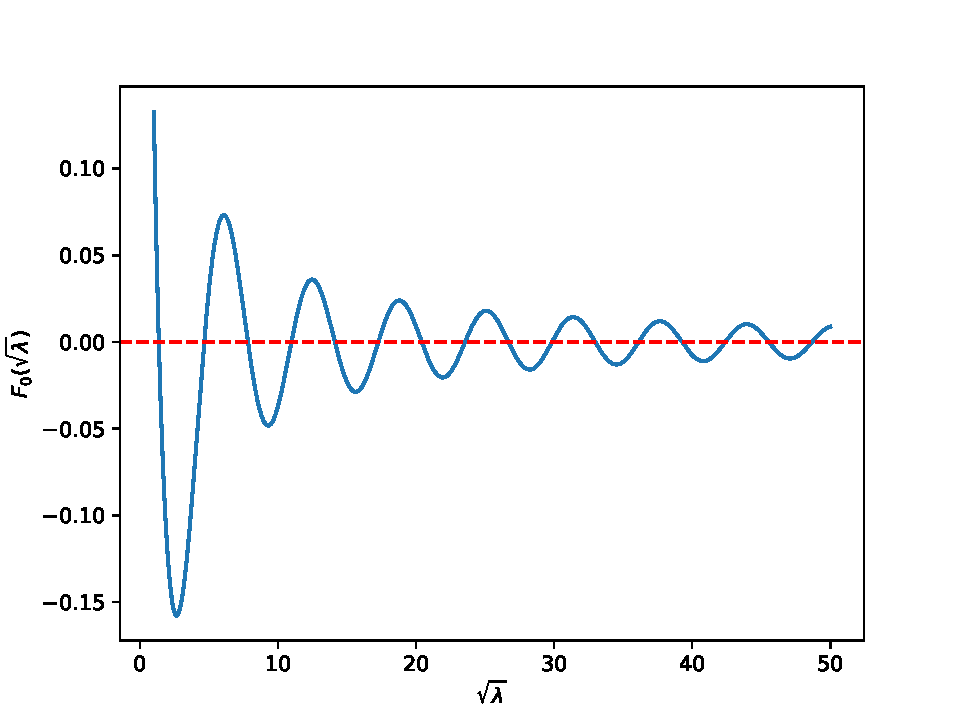
\includegraphics[width=0.8\textwidth]{F0}
\caption{It is straightforward to evaluate the cross-product of
Bessel functions Eq.~\ref{eq:eigenfunction} by SciPy
library \cite{2020SciPy-NMeth}. \label{fig:F0}}
\end{figure}


After the numerical estimation of the $n-$th positive root
$\lambda_{0,n}$ of Eq.~\ref{eq:eigenfunction}, the next step is to
approximate $u(\hat r, \theta, \tau)$ with the first $1000$
eigenvalues and the discretized radius $\hat r$ and $\tau$. As
illustrated in Figure~\ref{fig:u}, the diffusion problem experiences a
rapid change in the very beginning, but then the evolution of $u$
becomes slower and slower. Finally, the initial shape of $u$ can not
be recognized anymore.

\begin{figure}
\centering
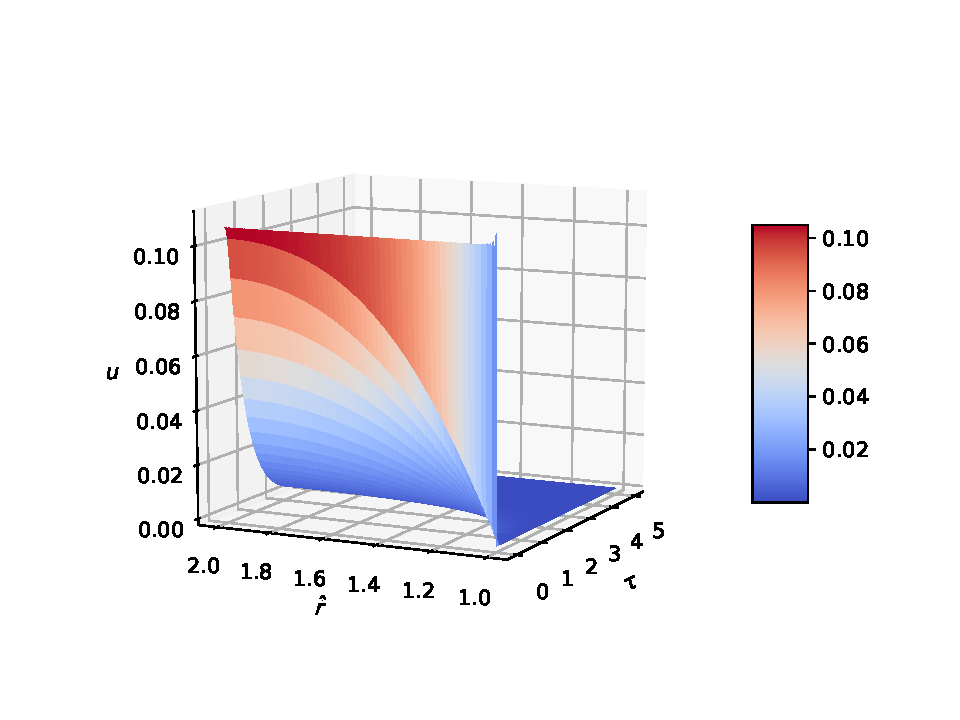
\includegraphics[width=\textwidth]{analytical_u}
\caption{When $\tau=0$, the approximated initial value of $u$ is about $0.106079414$ while the analytical result is $1/3\pi \approx 0.106103295$. The absolute error is $2.3881 \times 10^{-5}$. Moreover, the Gibbs phenomena \cite{fay2003gibbs} happened obviously near the discontinuity $\hat r = 0$ with the overshoots and undershoots because of the Fourier-Bessel series. \label{fig:u}}
\end{figure}

Before the numerical approximation of the convergent non-alternating
general Dirichlet series \cite{hardy2013general} $S(\tau)$, $S(0)$ is
evaluated firstly, and it can be represented as

\begin{equation}\label{eq:s0}
\begin{split}
S(0) &= \sum_{n=1}^{\infty} \frac{4}{\mu^2 - 1} \frac{1}{\lambda_{0,n} \bigg\{\bigg[\frac{J_0(\sqrt{\lambda_{0,n}})}{J'_0(\mu\sqrt{\lambda_{0,n}})}\bigg]^2 -1\bigg\}}\\
&= \sum_{n=1}^{\infty} c_n
\end{split}
\end{equation}

As displayed in Figure~\ref{fig:s0_coeff}, the individual terms of the
series Eq.~\ref{eq:s0} are monotonically decreasing and approach to
$0$. Calculating the $1000-$th partial sum directly, $S(0)$ is
$0.9998649050990541$ to $16$ decimal places with $3$ digit
accuracy. However, Aitken’s method can speed up the convergence rate
of the partial sum sequence and improve the accuracy of the estimation
by constructing a new series. Moreover, it does not matter whether the
series is alternating or not. Aitken's acceleration is

\begin{equation}\label{eq:Aitken_method}
A^{(1)}_n = s_{n+1} - \frac{(s_{n+1} - s_n)^2}{s_{n+1} - 2s_n + s_{n-1}}
\end{equation}

where  $s_n$,  $n=1,  2,  3,  ...$,  is  the  $n-$th  partial  sum  of
Eq.~\ref{eq:s0}, and  $(s_{n-1}, s_n,  s_{n+1})$ are  three successive
partial  sums.   The  process   can  be   repeated  for   the  further
speed-up.  For example,  apply Eq.~\ref{eq:Aitken_method}  on the  new
series $A^{(1)}$  to generate  $A^{(2)}$, on  the series  $A^{(2)}$ to
obtain $A^{(3)}$, etc.

As displayed in Figure~\ref{fig:partial_sum}, instead of adding $1000$
terms of Eq.~\ref{eq:s0} directly, the result of sequence
transformation by Aitken's method is more precise, which is
$0.9999812339391291$ to $16$ decimal places with $4$ digit
accuracy. The error using Aitken's acceleration is $7.2$ times smaller
than simply using the partial sums.


Similarly, when $\tau > 0$, estimating $S(\tau)$ and $\langle \tau \rangle$ in
Eq.~\ref{eq:annulus_analytical_s} by Aitken's acceleration, shown in
Figure~\ref{fig:numerical_approxi_s}, for validating the research
methodology in the next chapter.



\begin{figure}
  \begin{subfigure}{0.9\textwidth}
  \centering 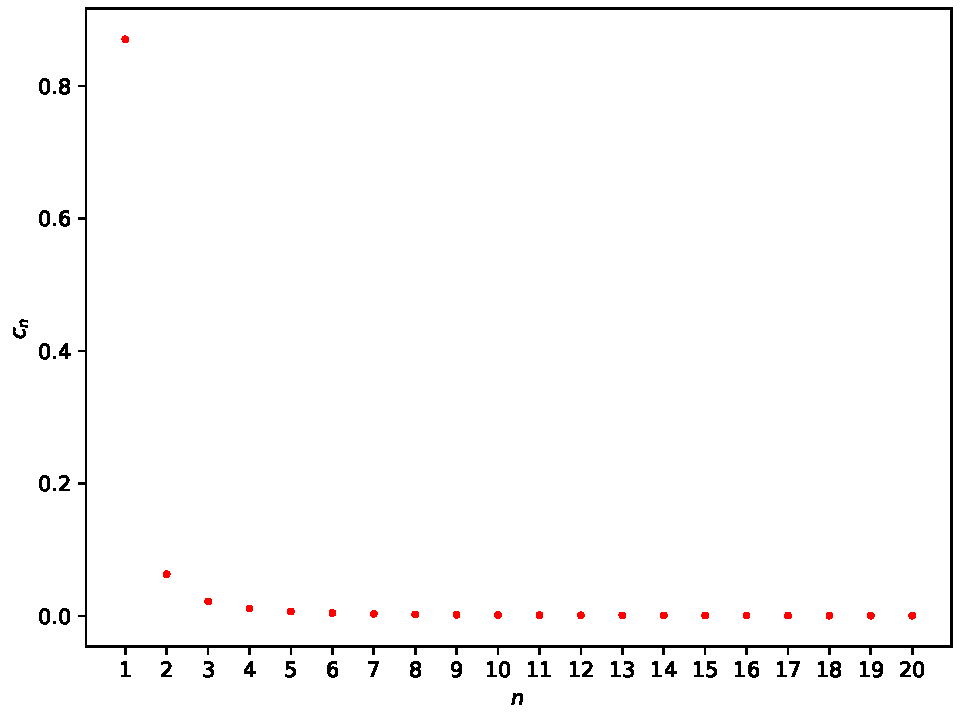
\includegraphics[width=0.8\textwidth]{coeff}
  \caption{The first $20$ terms of the series Eq.~\ref{eq:s0} are convergent and tend to zero. \label{fig:s0_coeff}}
  \end{subfigure}
  \begin{subfigure}{0.9\textwidth}
  \centering
  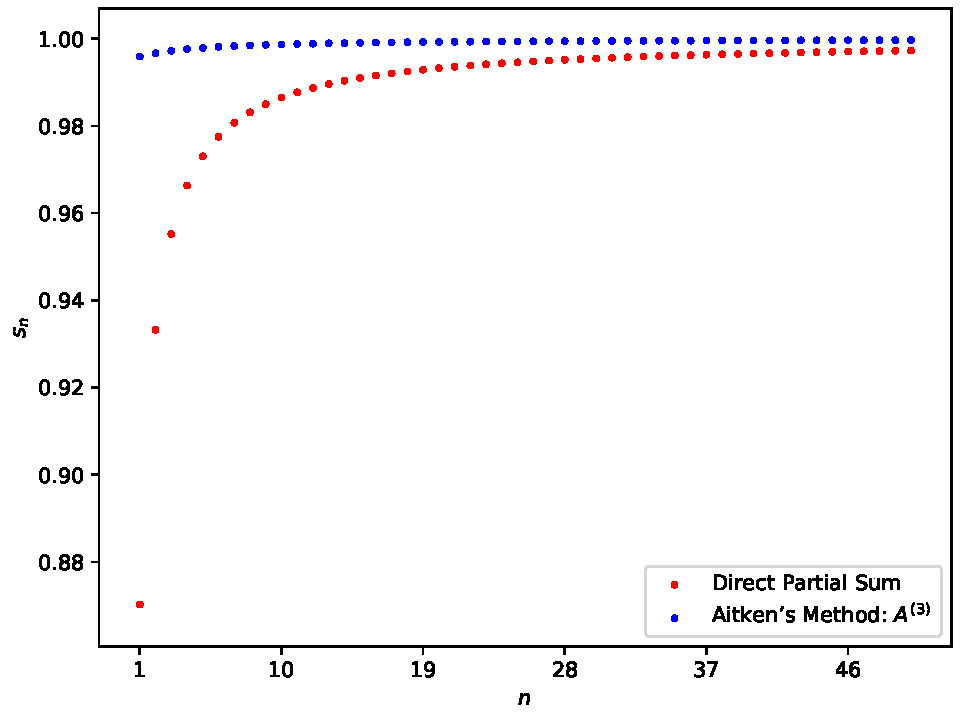
\includegraphics[width=0.8\textwidth]{partial_sum_coeff}
  \caption{The sequence of the partial sums of the series Eq.~\ref{eq:s0} tends to a real limit $1$. Compared with calculating the sum directly, $A^{(3)}_n$ converges more rapidly and approaches closer to $1$. \label{fig:partial_sum}}
  \end{subfigure}
  \caption{$S(0)$ is approximated by the direct summation and Aitken's acceleration. \label{fig:estimate_s0}}
\end{figure}



\begin{figure}
\centering
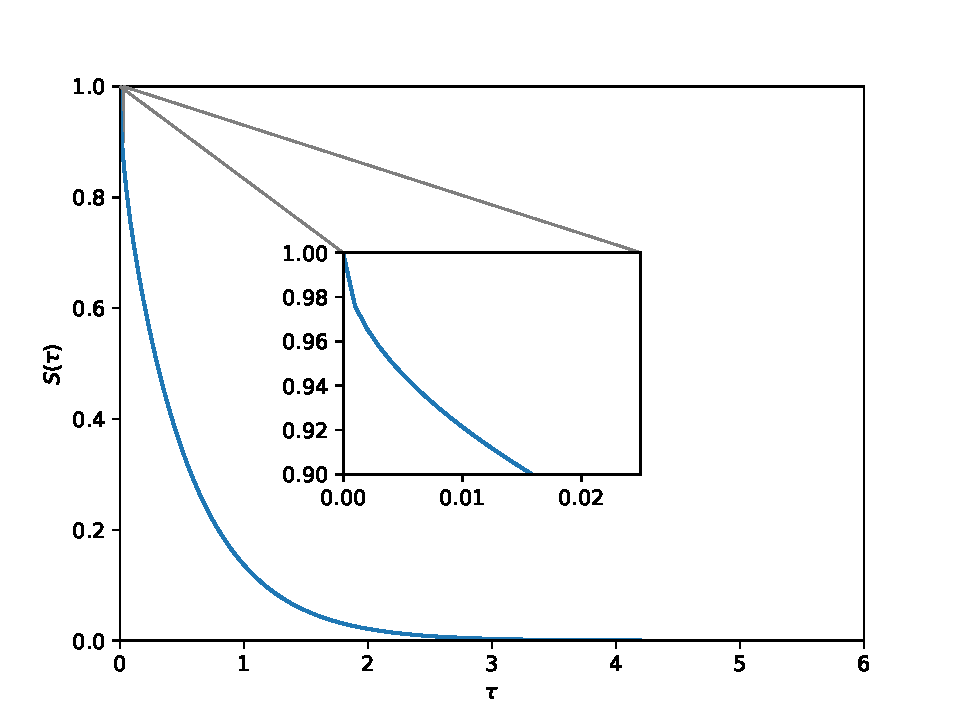
\includegraphics[width=0.8\textwidth]{analytical_s}%
\caption{The asymptotic behaviours of survival probability $S(\tau)$ is approximated by the Aitken's acceleration. $S(\tau)$ monotonously decreases from 1 at $\tau=0$ to $0$ as $\tau$ goes to infinity. Moreover, the approximation of analytical mean first-passage time $\langle \tau \rangle$ equals $0.47339248149521174$..\label{fig:numerical_approxi_s}}
\end{figure}




